\documentclass[../main/main]{subfiles}

\setcounter{chapter}{0}
\setcounter{page}{1}
\begin{document}

\chapter{序論}
\pagenumbering{arabic}

\section{研究背景}

\quad 近年,様々な進化計算(Evolutionary Computation, EC)手法が提案されている.
進化計算とは自然界の慣わしを工学的に模倣した最適化アルゴリズムの総称で,多点探索や関数の勾配情報が必要ないといった特徴から,多目的最適化に有効な手法であることが知られている.
進化計算の中でも特に多目的最適化に焦点を当てた手法は進化的多目的最適化アルゴリズム(Evolutionary Multiobjective Optimization Algorithms, EMOAs)と呼称される.
様々なEMOAが提案されているが,その中でも実数値遺伝的アルゴリズム(Real-Coded Genetic Algorithms; RCGAs; 実数値GA)の研究が盛んに行われており,実際の設計問題においてもその有効性が示されている\cite{Chiba2005,Oyama2010}.

実数値GAはバイナリ型遺伝的アルゴリズム(Binary-Coded Genetic Algorithms, BCGAs)と異なり,設計変数は0,1のバイナリビット列でなく実数値配列となる.
一般的に,実数値GAを用いた最適化では設計変数に連続値を仮定した実数値で取り扱うため,設計変数の有効桁数や離散化に関してユーザが意識することは少なく,計算機の取り扱える最大桁数を用いて最適化を行うことが多い.
しかし,現実の設計最適化問題では設計変数は実現性の観点から,離散値となったり有効桁数が設けられる場合が多い.
実数値GAをそのような設計問題に適用する場合,最終的に得られた解の設計変数を離散値に近似するか,設計変数を最適化のプロセスの途中で修正する必要がある.
設計変数を最適化のプロセスの途中で修正する場合,個体評価前に実際の設計変数の値を修正するか,仮想的に離散化して評価することが考えられるが,設計変数の離散化が実数値GAの探索性能に与える影響については,これまで十分に議論が行われていない.
また,現実の設計最適化問題では,目的関数や制約条件の評価に大きな計算資源を必要とする場合があり,産業界ではより少ない評価回数で効率的に探索することができる手法が求められている.

先行研究\cite{近藤2015}では,離散値が実数値GAの探索性能にどのような影響を与えるかを明らかにするため,代表的な実数値GAであるNon-dominated Sorting Genetic Algorithm II (NSGA-II)\cite{Deb2002Fast}と3つのベンチマーク問題を用いて,数値実験による評価を行った.
その結果,設計変数を粗く離散化するほど収束性が向上するが,問題によっては解の多様性が失われてしまう可能性があることが分かった.
しかしながら,他の実数値GAやベンチマーク問題,実際の設計問題においても同様の現象が確認できるかなど,未だ不明確な部分も多い.
また,問題に応じて各設計変数を適切に離散化することができれば,解の多様性を維持しながらも収束性を高められる可能性があるが,最適化を行う前に適切に離散化することは難しく,設計変数の離散化の有効な活用法が課題となっていた.
以上のことから,先行研究の結果の一般性の確認と共に,設計変数の離散化の有効な活用方法を検討することが必要であると考えられる.

%実際の多目的設計問題を対象とする場合,設計問題を構成する変数が離散値を取ることが多い.
%通常,実数値GAでは連続値を仮定した設計変数を用いて取り扱っているため,離散値を用いた場合,従来の計算結果とは異なる結果が出ることが考えられる.
%
%先行研究\cite{}では,離散値が実数値GAの探索性能にどのような影響を与えるかを明らかにするため,代表的な実数値GAであるNSGA-IIと3つのベンチマーク問題を用いて,数値実験による評価を行った.
%その結果,設計変数を粗く離散化するほど収束性が向上するが,問題によっては解の多様性が失われてしまう可能性があることが分かった.
%しかしながら,他の実数値GAやベンチマーク問題,実際の設計問題においても同様の減少が確認できるかなど,未だ不明確な部分も多い.
%したがって,先行研究の結果の一般性の確認と共に,設計変数の離散化の有用な活用方法を検討することが必要であると考えられる.



%そこで,本研究では設計変数の離散化が実数値GAの探索性能に与える影響を幅広く評価することを目的とする.

%しかしながら,実際の設計問題では目的関数や制約条件の評価に大きな計算資源を必要とする場合があり,パレート最適解(非劣解)集合を一度に得ることができるものの,最適解を得るまでに必要な計算時間が課題となっており,更なる効率的な探索手法が求められている.
%
%RCGAはバイナリ型遺伝的アルゴリズム(Binary-Coded Genetic Algorithms, BCGAs)と異なり,設計変数は0,1のバイナリビット列でなく実数値配列となる.
%一般的に,RCGAを用いた最適化では設計変数に連続値を仮定した実数値で取り扱うため,設計変数の有効桁数や離散化に関してユーザが意識することは少なく,計算機の取り扱える最大桁数を用いて最適化を行うことが多い.
%しかし,現実の設計最適化問題では設計変数は実現性の観点から,離散値となったり有効桁数が設けられる場合が多い.
%RCGAをそのような設計問題に適用する場合,最終的に得られた解の設計変数を離散値に近似するか,設計変数を最適化のプロセスの途中で修正する必要がある.
%設計変数を最適化のプロセスの途中で修正する場合,個体評価前に実際の設計変数の値を修正するか,仮想的に離散化して評価することが考えられるが,そもそも設計変数の離散化がRCGAの探索性能に与える影響については,これまで十分に議論が行われていなかった.
%
%BCGAにおいては,設計変数のビット長を短くするほど解の収束速度が向上することが報告されている\cite{jaimes}.
%これは,設計変数のビット長を短くすることで,設計変数空間が粗く離散化され,探索空間の縮小に繋がるためだと考えられている.
%\ref{discretization_sample}は,異なるビット長を用いた際の探索空間の違いを示しており,格子点が各ビット長を用いた際の探索点を表している.
%\ref{discretization_sample}からわかるようにビット長を短くすることで,設計変数空間が粗く離散化され探索空間が減少していることがわかる.
%この性質を活かし,BCGAではビット長を探索の中で動的に変化させることで探索速度を向上させる手法が提案されている\cite{jaimes,kim}.
%
%\begin{figure}[htbp]
%\begin{center}
%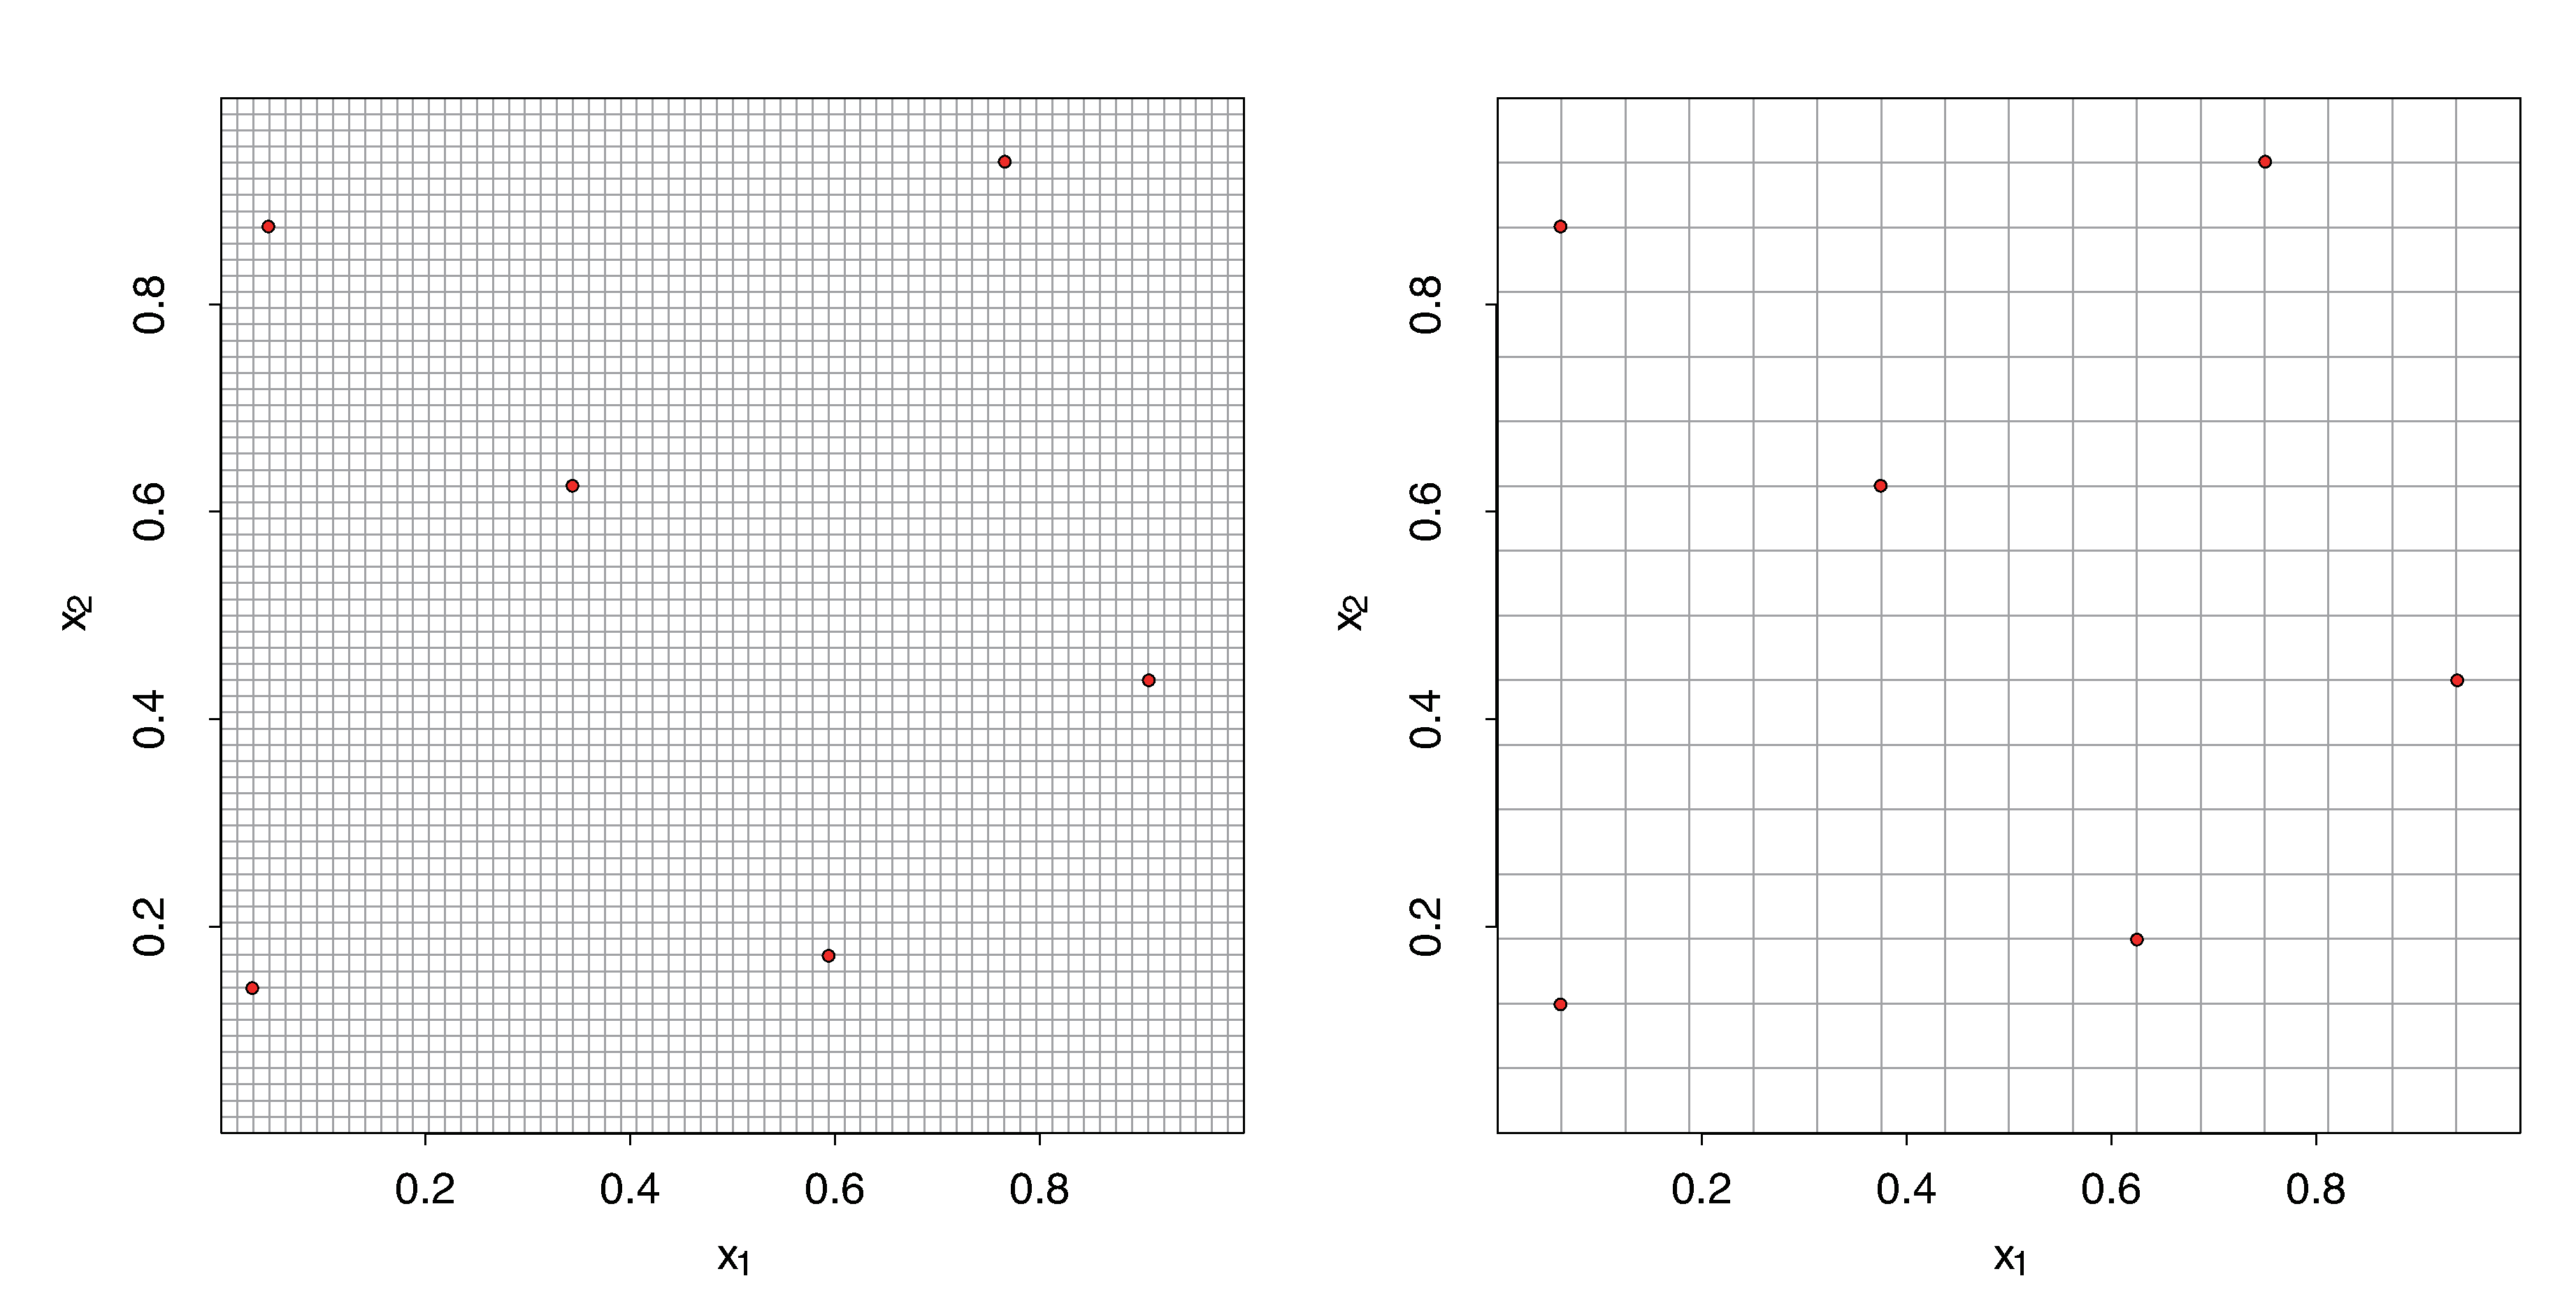
\includegraphics[width=0.9\linewidth]{../figures/discretization_sample.eps}
%\end{center}
%\caption{離散化による探索空間のイメージ図(左:ビット長6を用いた0-1の二変数の探索範囲 右:ビット長4を用いた0-1の二変数の探索範囲)}
%\label{discretization_sample}
%\end{figure}
%
%
%RCGAではBCGAのように設計変数を動的に離散化する手法の検討は進んでいない.
%設計変数の離散化がRCGAの探索性能に与える影響については,Kondoらの先行研究\cite{kondo}により代表的な実数値GAであるNSGA-II\cite{}を用いて,設計変数の離散化が探索に及ぼす影響が評価されている.
%その結果の一部を\ref{pre_dtlz3},\ref{pre_dtlz4}に示す.
%
%\ref{pre_dtlz3}はDTLZ3と呼ばれるベンチマーク問題において,粗い離散化を行った設計変数を用いた場合と連続値に近い設計変数を用いた場合それぞれにおいて同じ評価回数で得られた非劣解の分布を示したものである.
%各軸はそれぞれ目的関数を示しており,青色の点は非劣解を示している.
%この問題は3目的の最小化問題として定式化されているため,図中の原点方向が最適化方向であり,原点に近い点ほど優れた個体を表している.
%\ref{pre_dtlz3}より,粗く離散化を行った設計変数を用いた場合のほうが明らかに最適化方向である原点に近い個体が生成されている.
%このことから,DTLZ3では粗く設計変数を離散化することで,解の収束性が向上することがわかった.
%この傾向は他の多くのベンチマーク問題においても確認されている.
%
%\begin{figure}[htbp]
%\begin{tabular}{cc}
%\begin{minipage}{0.49\hsize}
%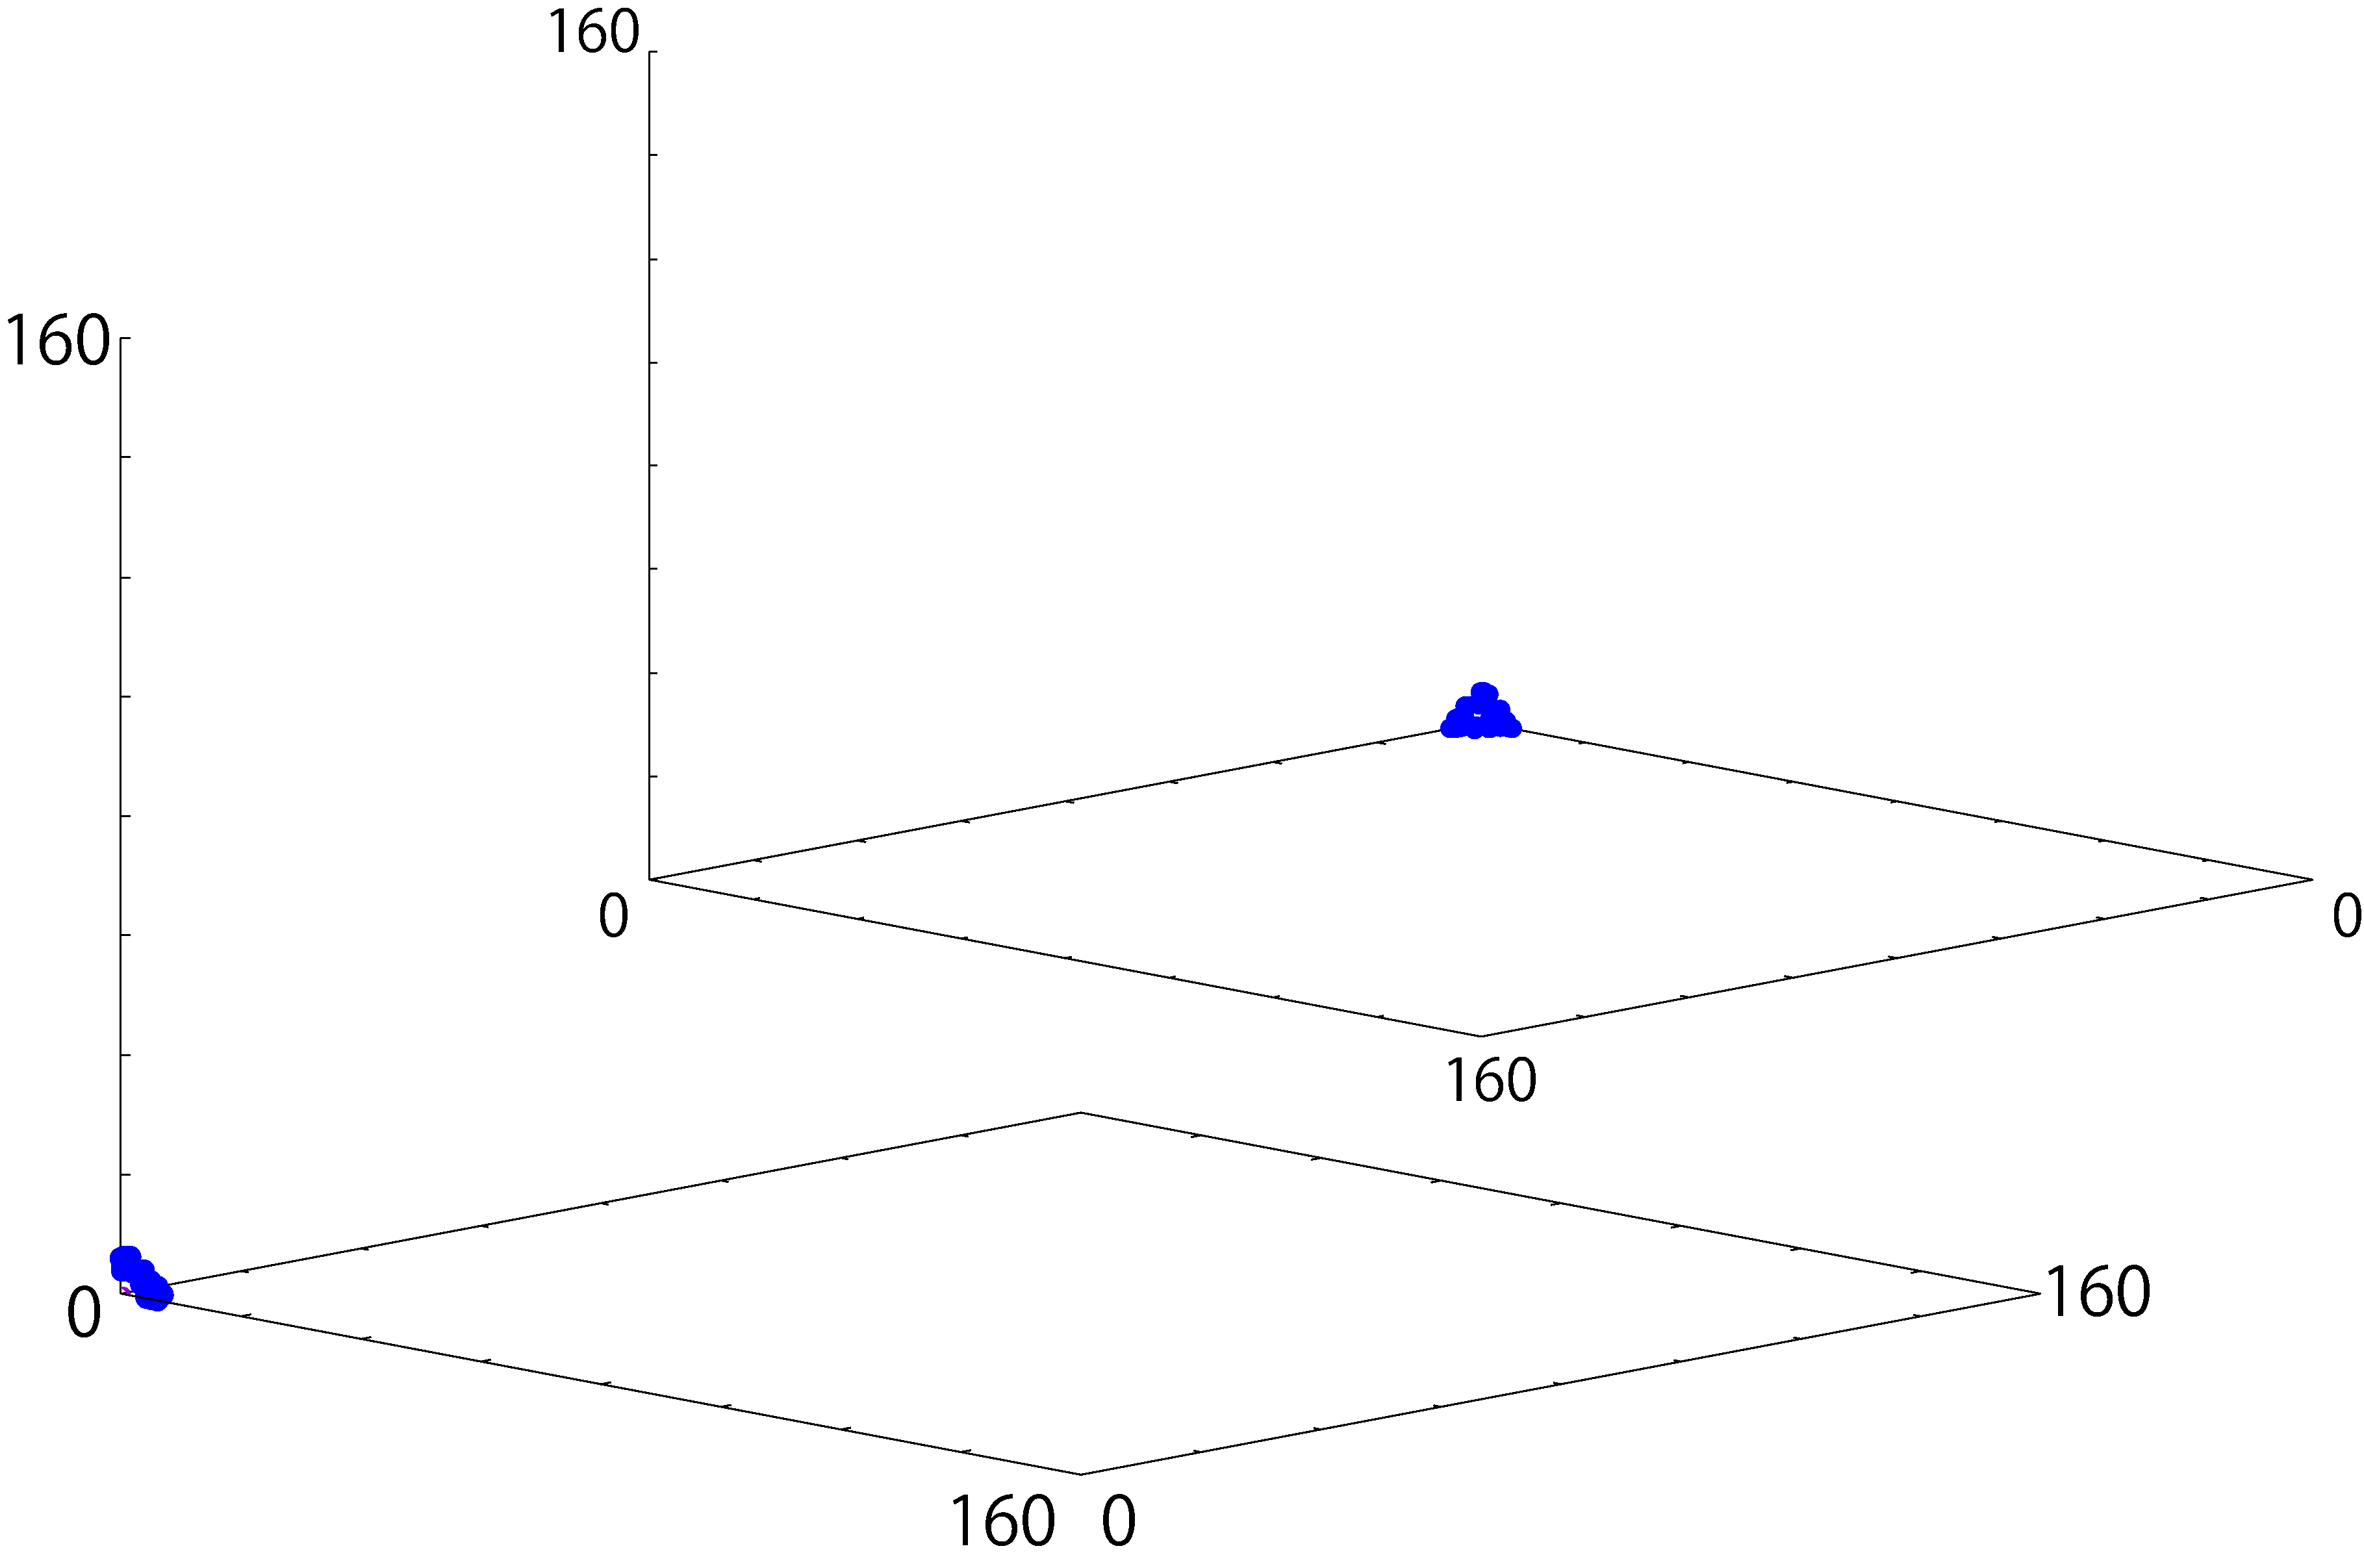
\includegraphics[width=0.9\linewidth]{../figures/dtlz3_digi2_double.pdf}
%\begin{center}
%{\footnotesize (a) 粗く離散化を行った設計変数を用いた場合}
%\end{center}
%\end{minipage}
%\begin{minipage}{0.49\hsize}
%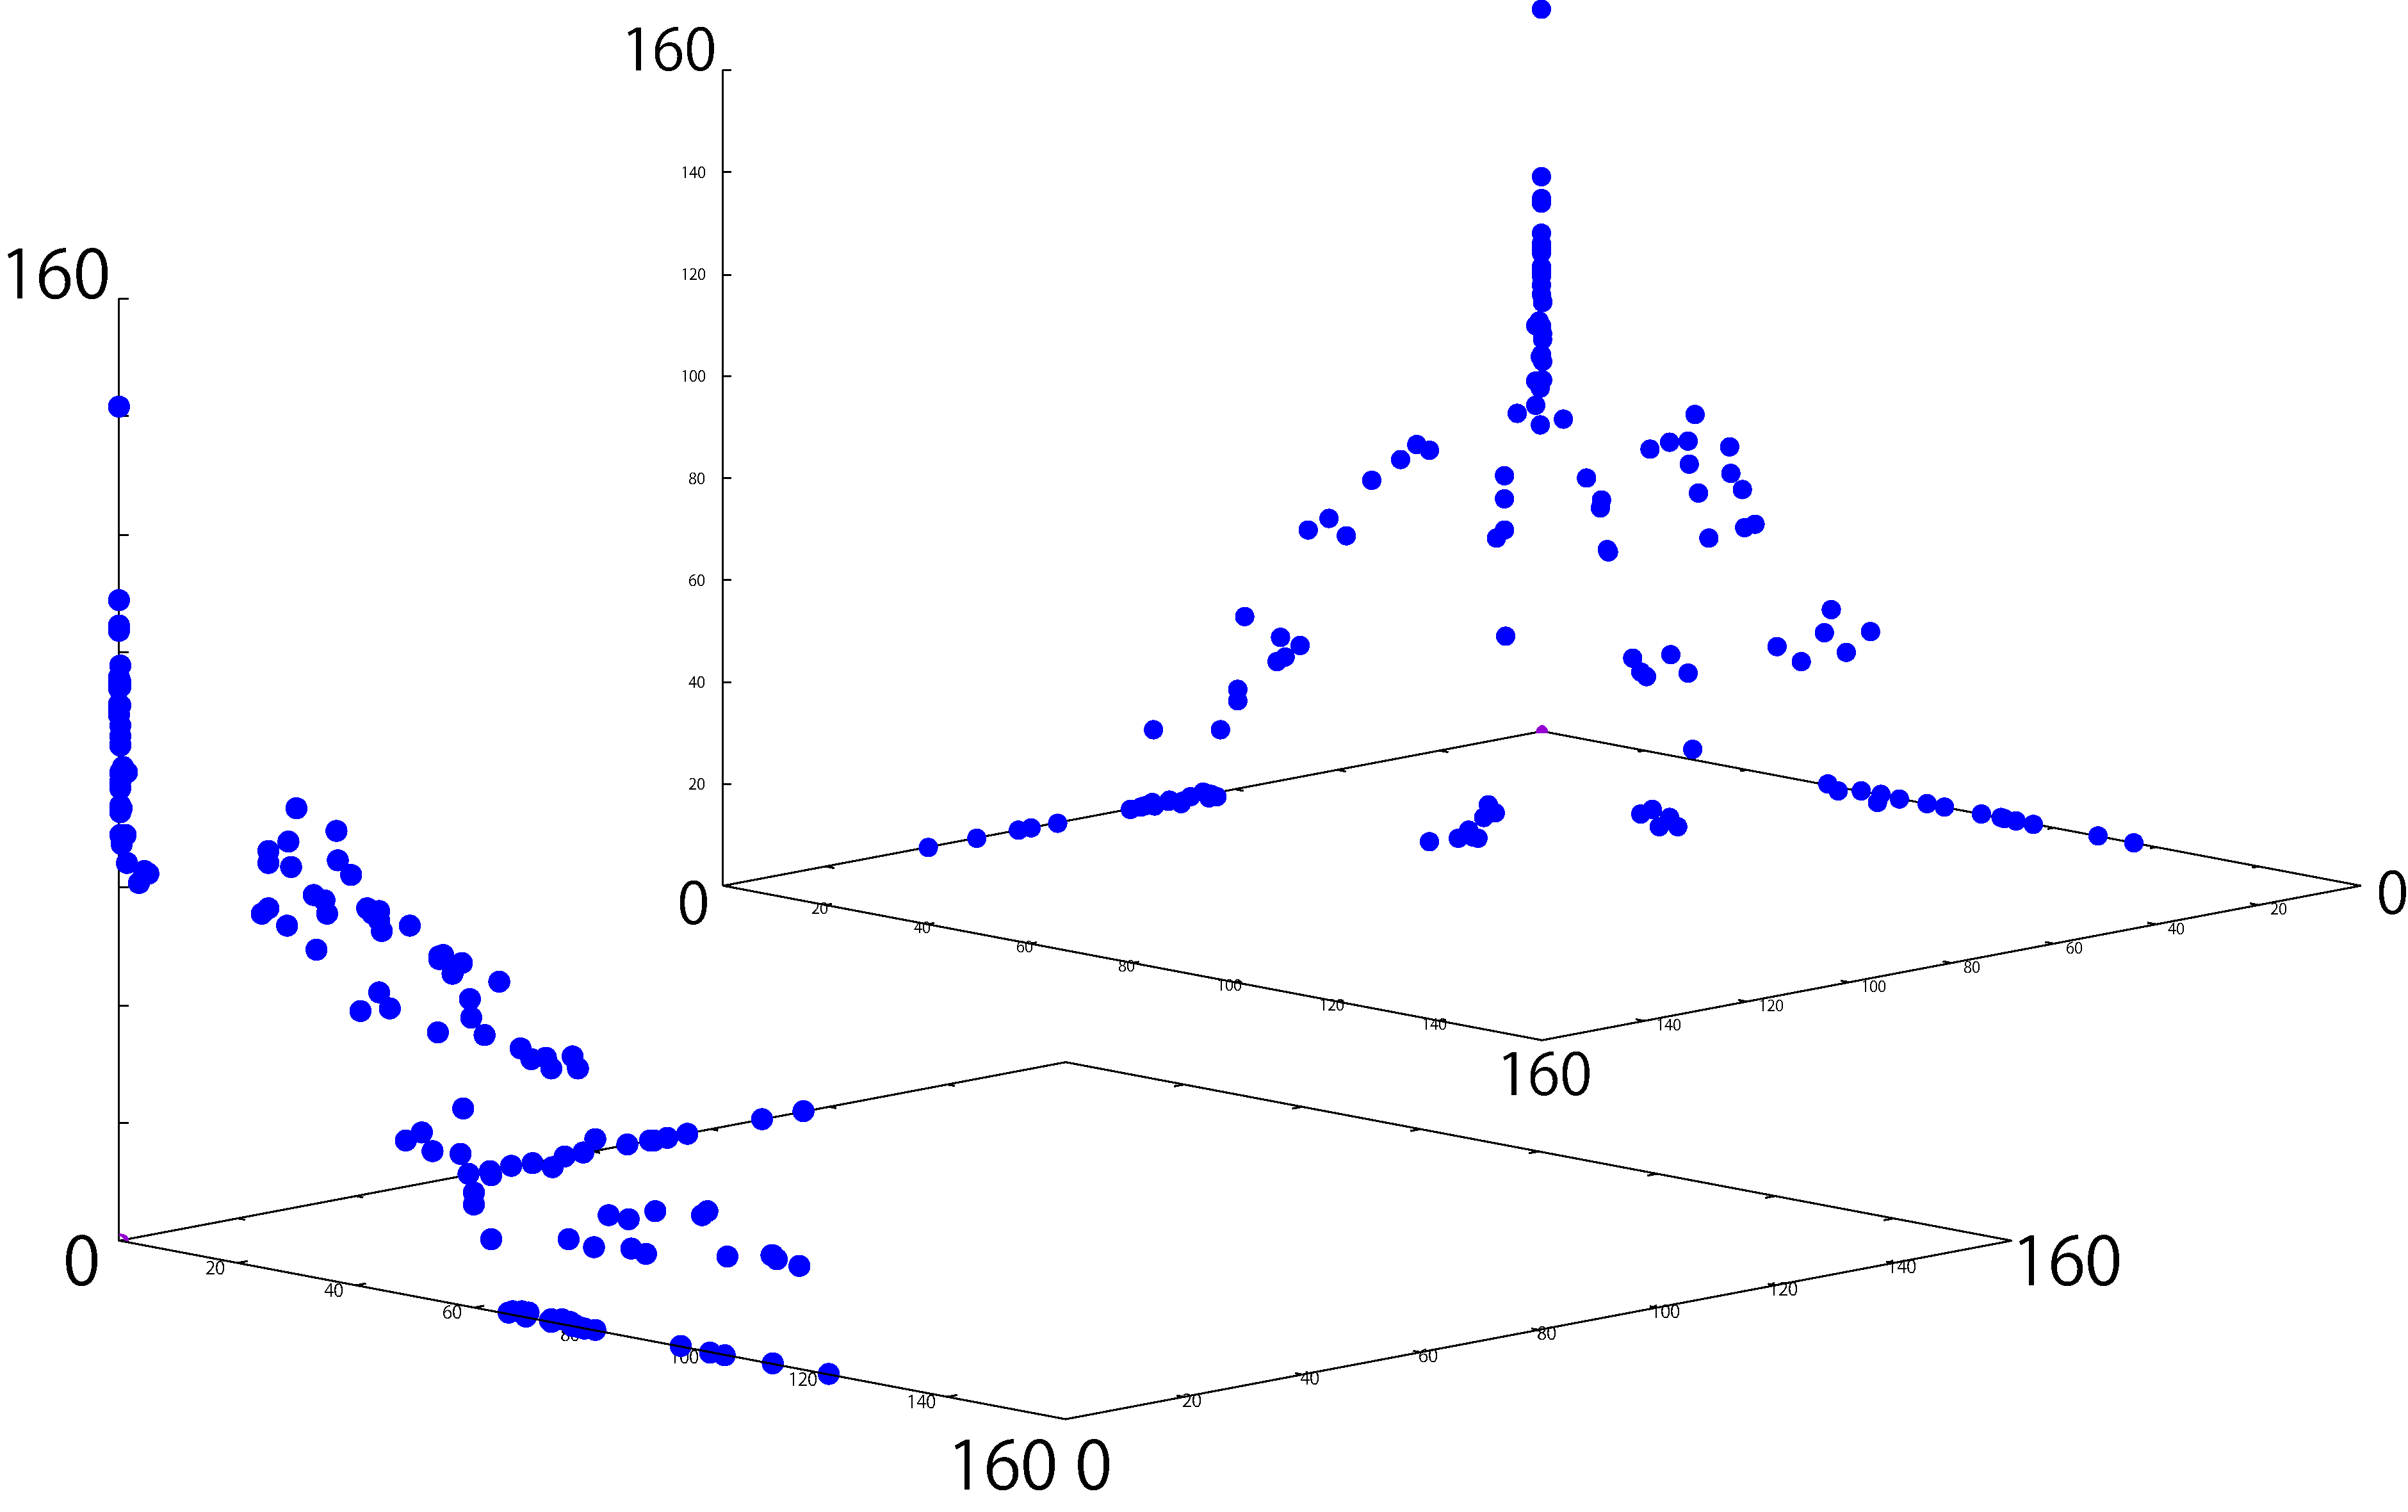
\includegraphics[width=0.9\linewidth]{../figures/dtlz3_digi16_double.pdf}
%\begin{center}
%{\footnotesize (b) 連続値に近い設計変数を用いた場合}
%\end{center}
%\end{minipage}
%\end{tabular}
%\caption{DTLZ3における設計変数の離散化の有無による非劣解の比較}
%\label{pre_dtlz3}
%\end{figure}
%
%
%\ref{pre_dtlz4}はDTLZ4と呼ばれるベンチマーク問題において,粗い離散化を行った設計変数を用いた場合と連続値に近い設計変数を用いた場合それぞれにおいて同じ評価回数で得られた非劣解の分布を示したものである.
%各軸はそれぞれ目的関数を,青色の点は非劣解を,紫の線は真のパレート最適解の形状を示したものである.
%この問題は3目的の最小化問題として定式化されているため,図中の原点方向が最適化方向であり,真のパレート最適解に近い点ほど優れた個体を表している.
%また,多目的最適化では,単に真のパレート最適解に近い解が得られるだけでなく,真のパレート最適解を覆うような多様な解が生成されることも求められる.
%\ref{pre_dtlz4}より,粗く離散化を行った設計変数を用いた場合は,真のパレート最適解に対して局所的にしか解が生成されておらず,解の多様性という観点では悪い結果となっている.
%一方で,連続値に近い設計変数を用いた場合は,真のパレート最適解を覆うように解が生成されており,解の多様性が良いことが分かる.
%このように,問題によっては設計変数を粗く離散化しすぎてしまうと,解の多様性が失われる可能性があることがわかっている.
%
%
%\begin{figure}[htbp]
%\begin{tabular}{cc}
%\begin{minipage}{0.49\hsize}
%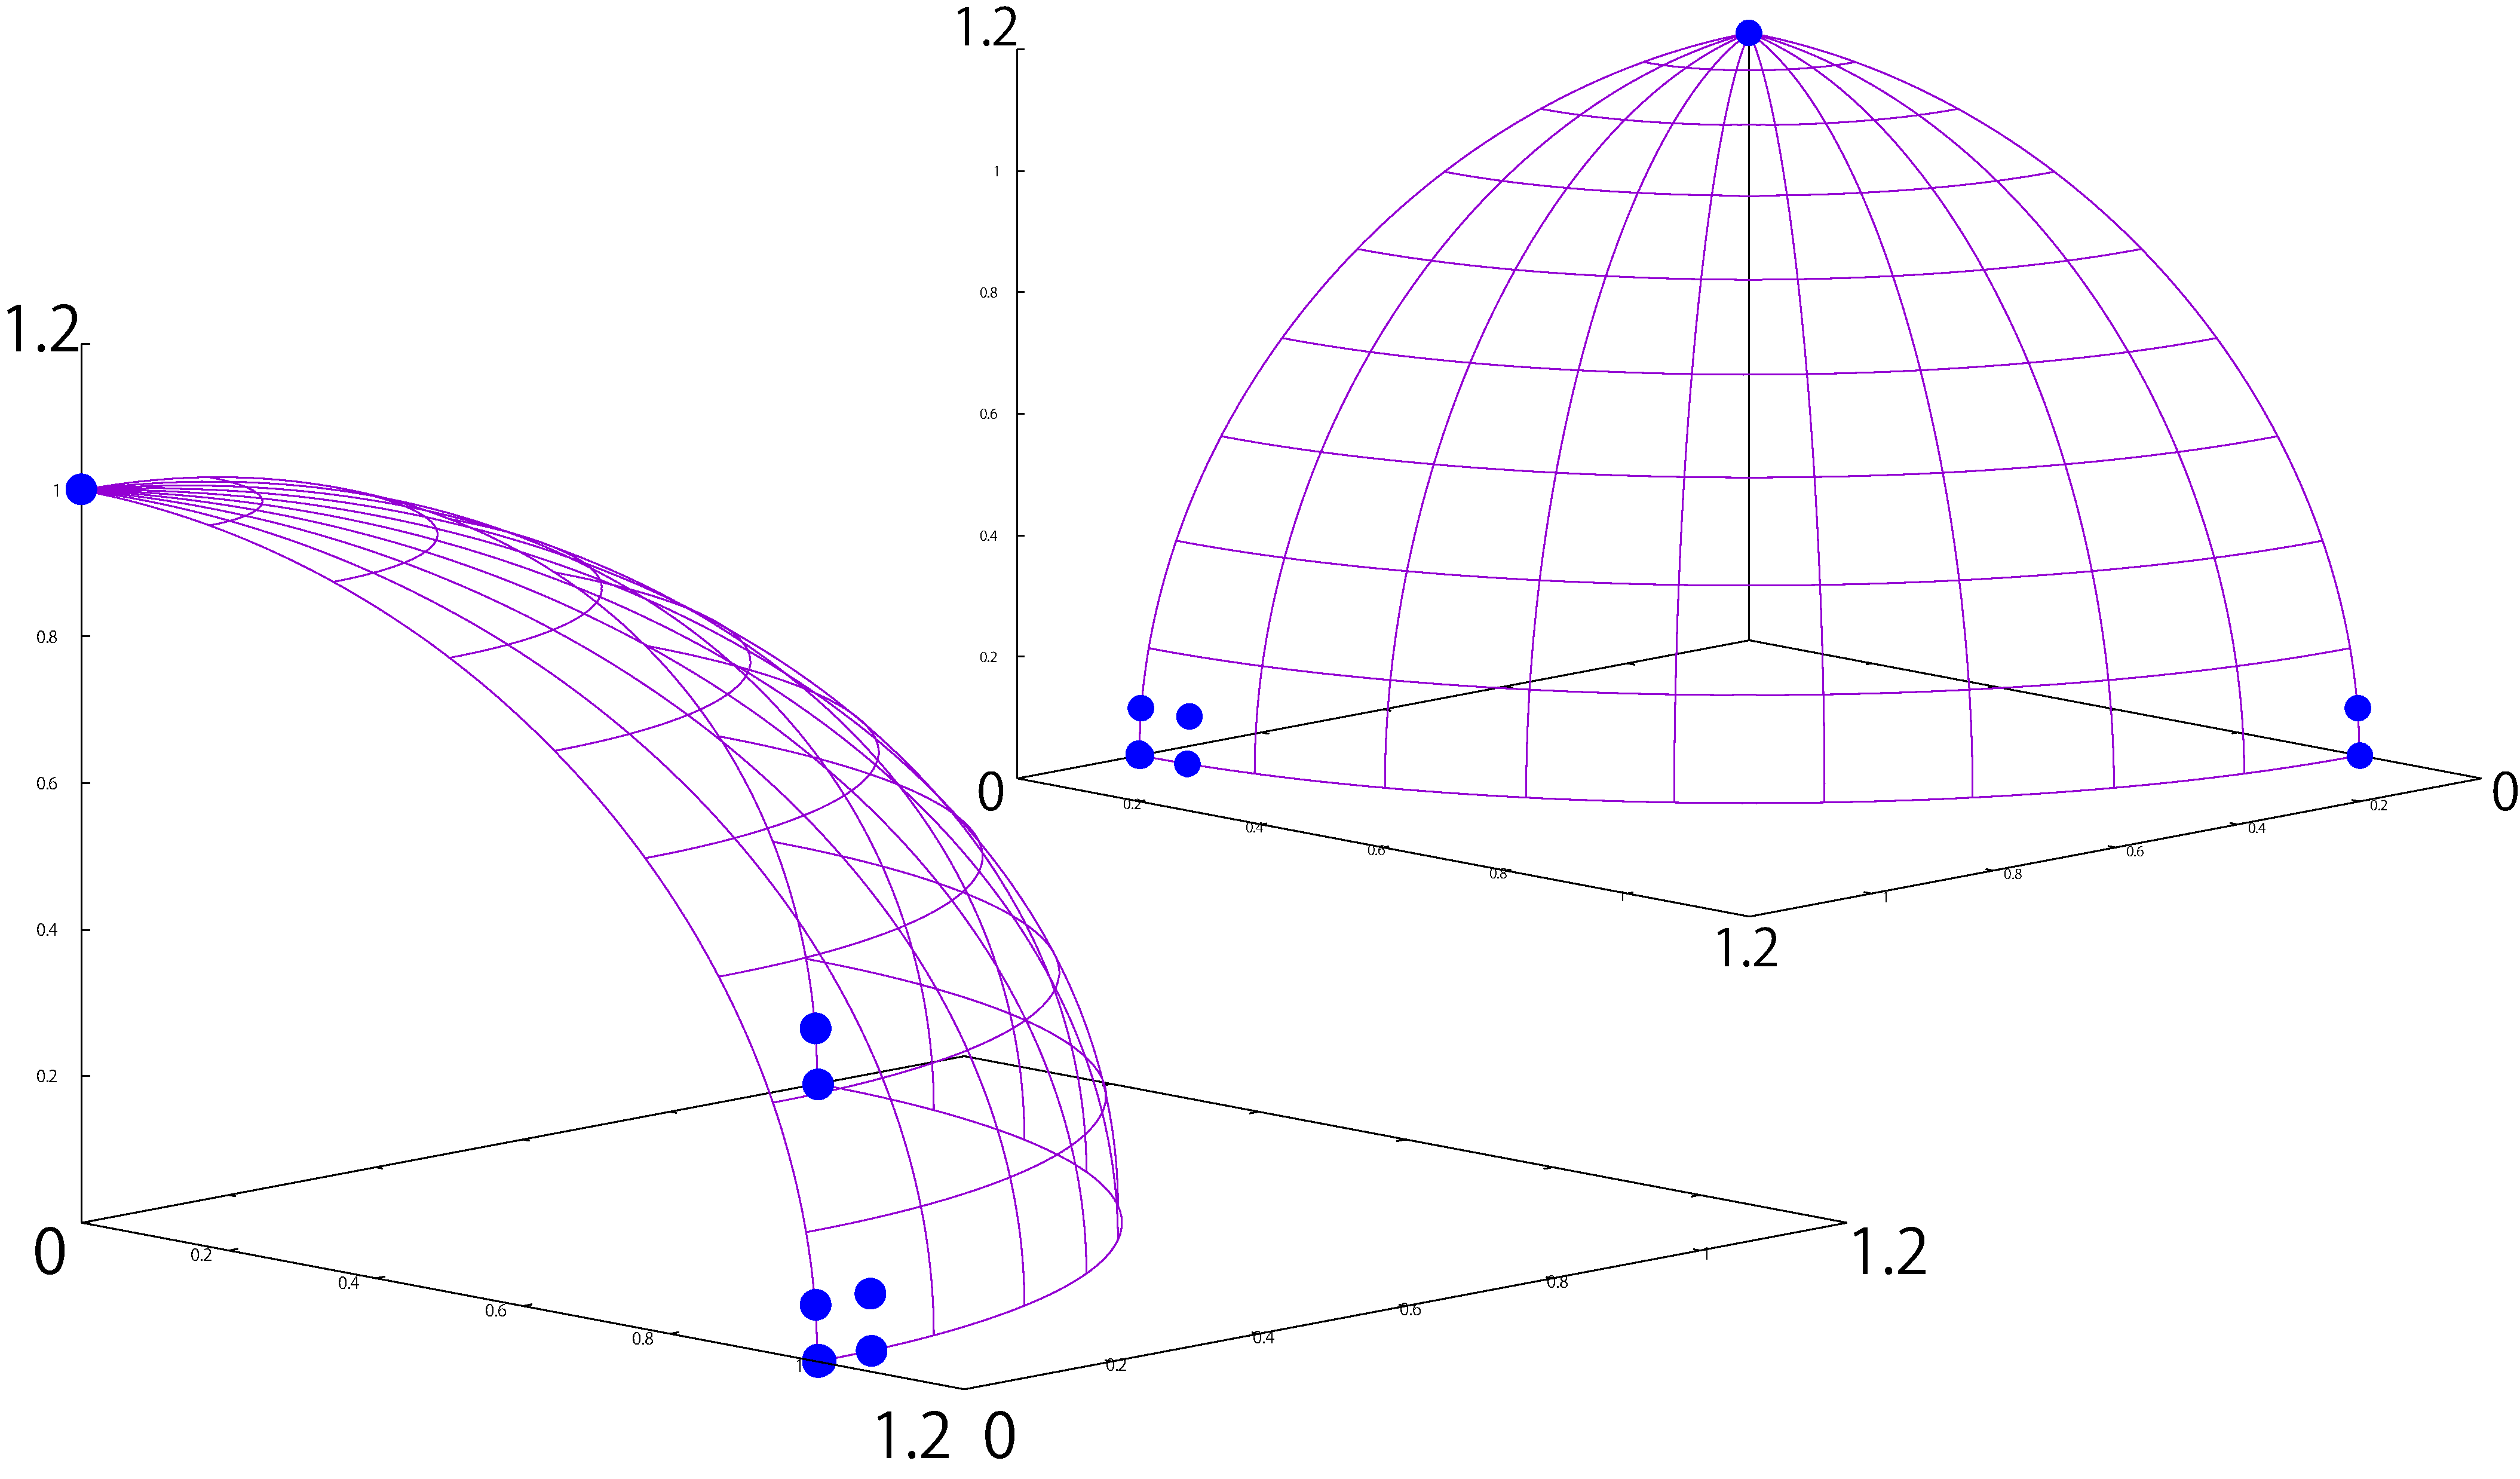
\includegraphics[width=0.9\linewidth]{../figures/dtlz4_digi2_double.pdf}
%\begin{center}
%{\footnotesize (a) 粗く離散化を行った設計変数を用いた場合}
%\end{center}
%\end{minipage}
%\begin{minipage}{0.49\hsize}
%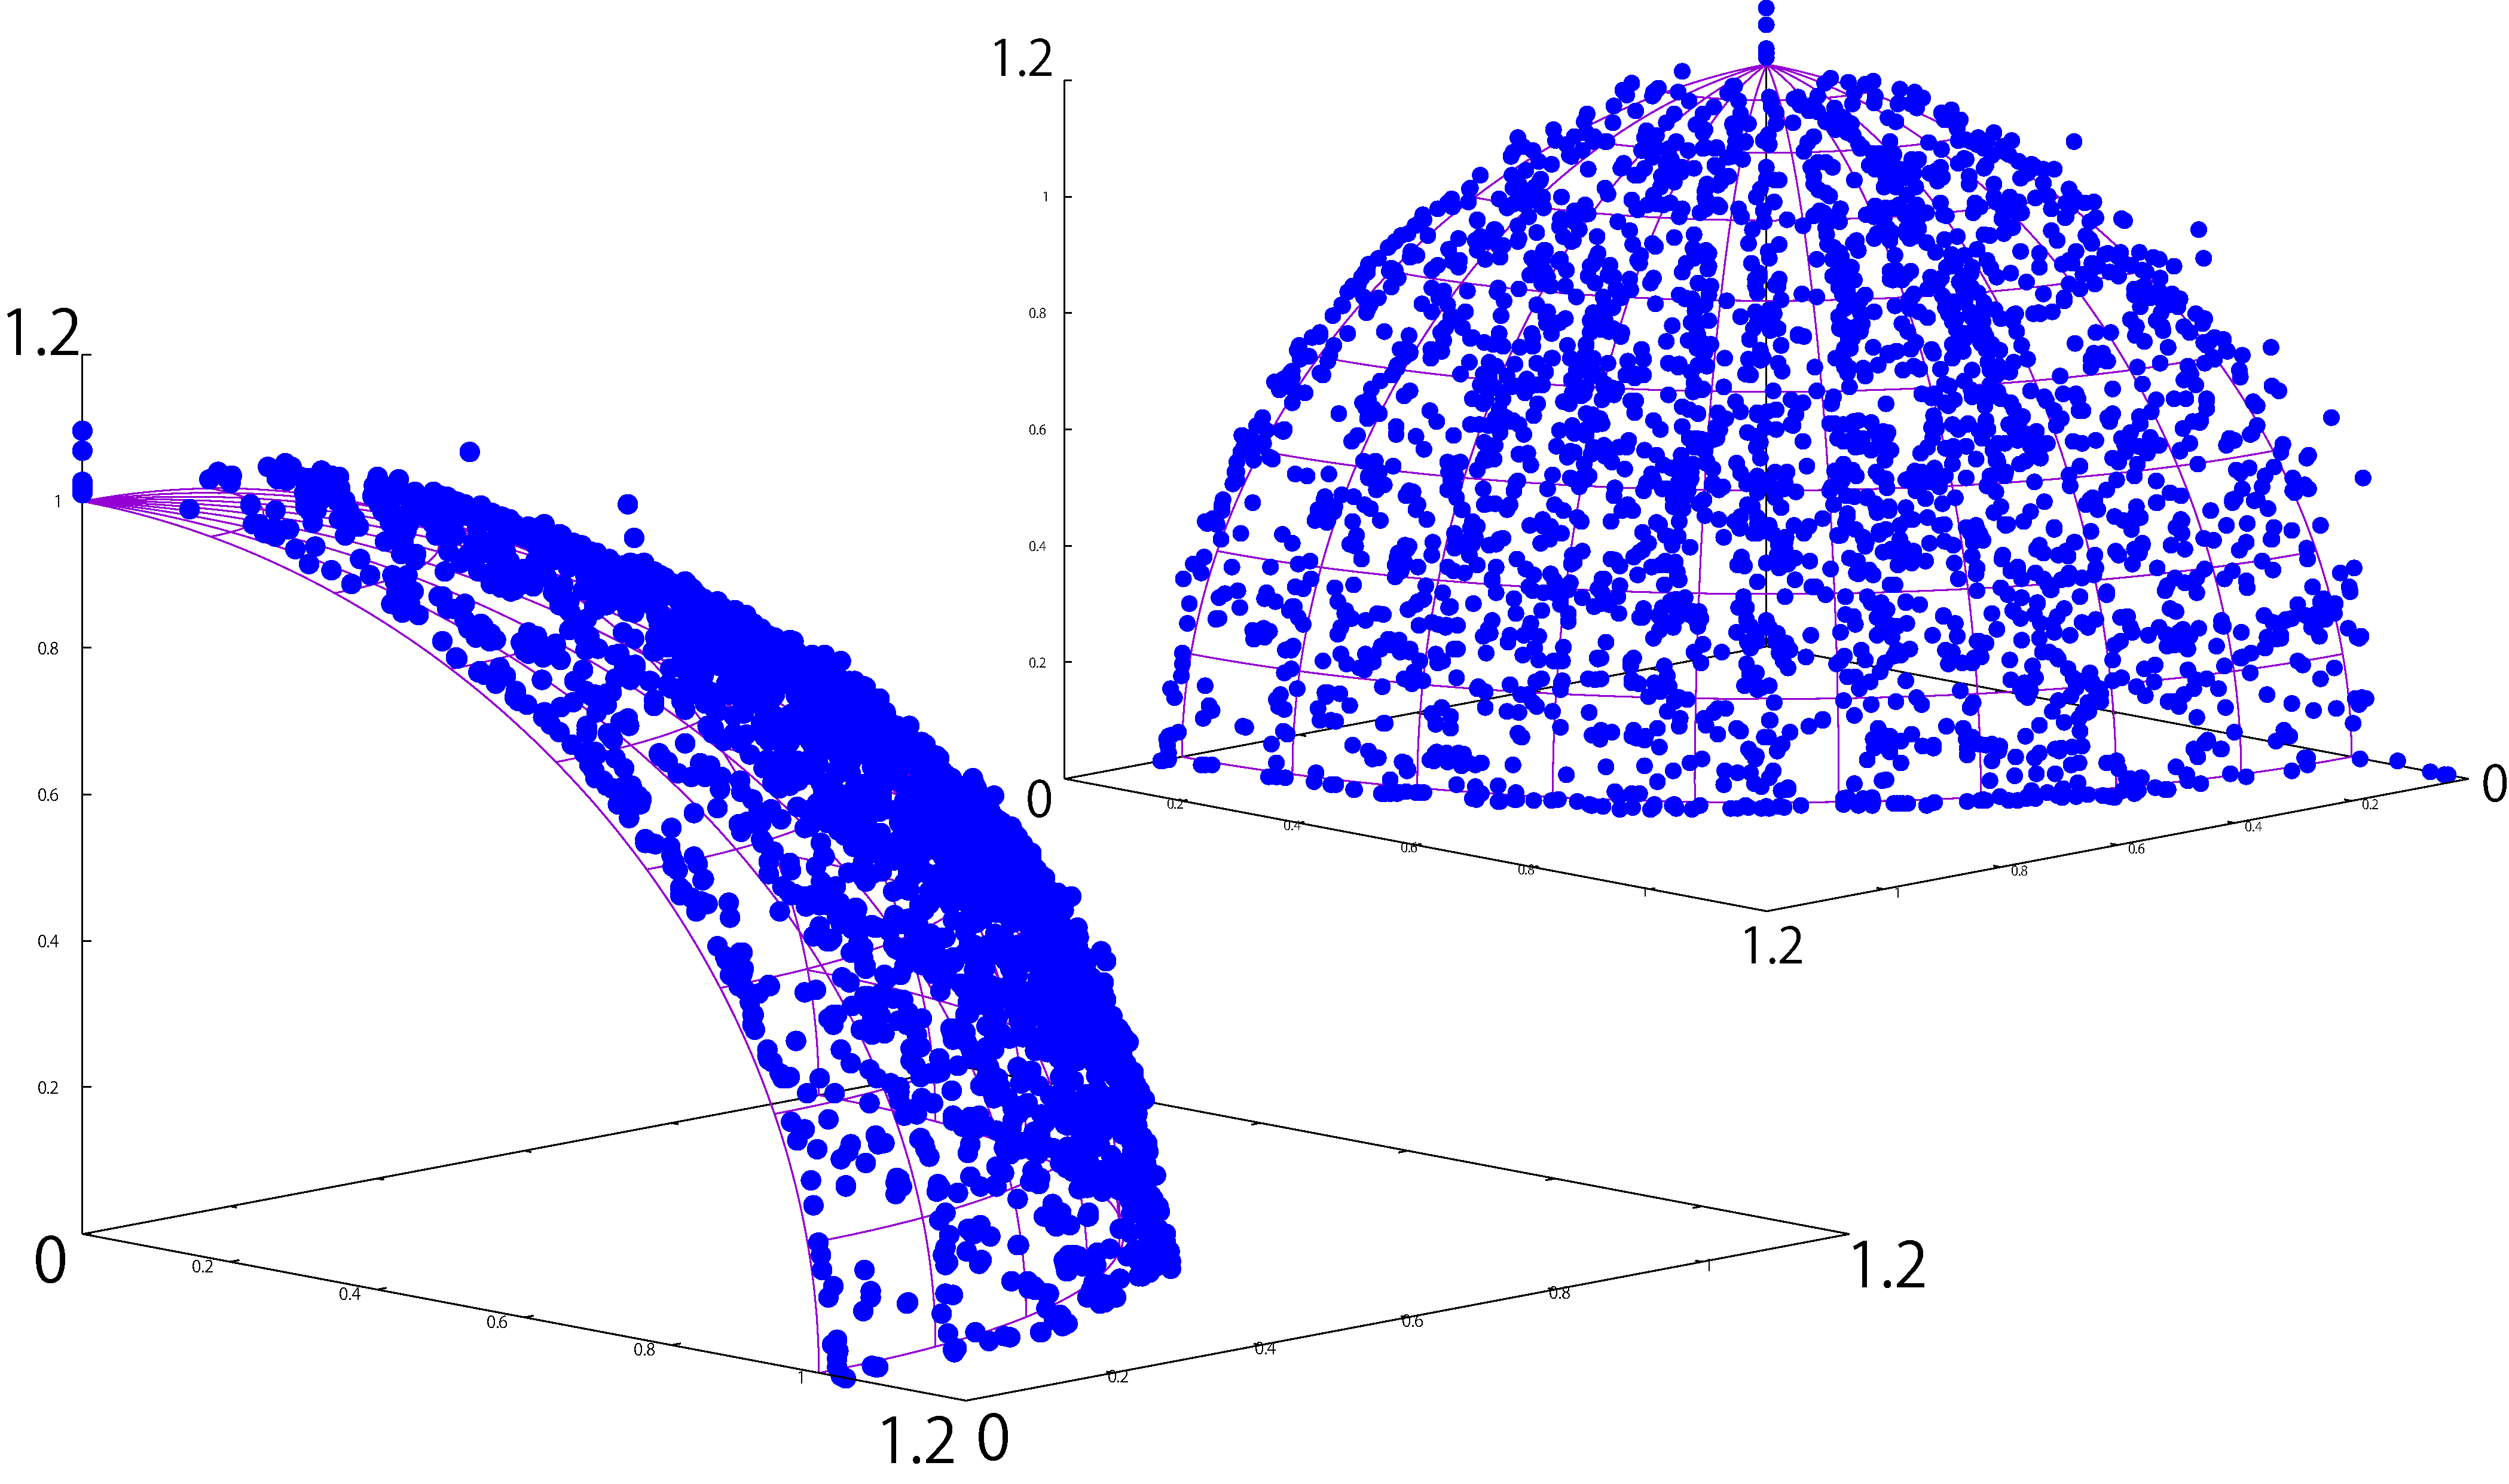
\includegraphics[width=0.9\linewidth]{../figures/dtlz4_digi16_double.pdf}
%\begin{center}
%{\footnotesize (b) 連続値に近い設計変数を用いた場合}
%\end{center}
%\end{minipage}
%\end{tabular}
%\caption{DTLZ4における設計変数の離散化の有無による非劣解の比較}
%\label{pre_dtlz4}
%\end{figure}
%
%以上の先行研究の結果から,問題によって各設計変数を適切に離散化することで,RCGAにおいても効率的に探索することが可能であると考えられる.
%
%しかしながら,最適化を行う前に各設計変数を適切に離散化することは難しく課題となっていた.

\section{研究目的}
\quad 本研究では,設計変数の離散化が実数値GAの探索性能に与える影響を幅広く検証し,その一般性を明らかにすることを目的とする.
また,その結果から設計変数の離散化の有効な活用方法の検討を進め,産業界で求められている効率的探索に繋がる手法の提案を行う.
ここでは,先行研究のNSGA-IIに加え,代表的実数値GAの一つであるMulti-objective Evolutionary Algorithm Based on Decomposition (MOEA/D)\cite{Zhang2007MOEAD}での検証を行い,実際の設計問題を模擬した Engineering 問題を含む19個のベンチマーク問題を用いて影響を評価する.
この結果から設計変数の離散化の活用法として,適応的離散化手法の提案を行う.
適応的離散化手法の性能評価においては,NSGA-IIに適用し,24個のベンチマーク問題を用いて,影響評価と同様に性能評価を行う.
%また,その結果から設計変数の離散化の活用法を考察し,効率的探索手法の提案に繋げる.
%\quad 上述した通り,問題によって各設計変数を適切に離散化することで,効率的に探索することが期待できるが,最適化を行う前に各設計変数を適切に離散化することは難しい.
%そこで,本研究では,RCGAにおける設計変数空間の適応的離散化手法を提案する.
%RCGAにおいて提案手法を用いて適応的に設計変数を離散化することにより,解の多様性を維持しながらも収束性を向上させられることが期待される.
%ここでは,各設計変数空間における解の分布状態を評価し,それを基に適応的に設計変数を離散化することを考える.
%RCGAとしてはNSGA-IIに提案手法を適用し,24個のベンチマーク問題を対象に提案手法の有効性を検証する.

\section{本論文の構成}
\quad 本論文は「設計変数の適応的離散化を用いた実数値GAの効率的探索手法の提案」と題し,全7章より構成されている.

第1章「序論」では,本研究を取り組むにあたっての背景と課題を説明し,本研究の目的を明らかにする.

第2章「多目的最適化」では,本研究で取り扱う多目的最適化について論じる.
 多目的最適化問題及び,多目的最適化における進化計算,遺伝的アルゴリズム,解の評価指標など,本研究に関わる内容を中心にまとめる.

第3章「関連研究」では,本研究で取り扱う「離散化」に関する多目的最適化の研究をまとめる.
また,離散化について影響評価を行った先行研究で残された課題を明らかにし,本研究の方向性について論じる.

第4章「設計変数の離散化による影響評価」では,先行研究で残された課題を解決するため,代表的な二つの実数値GAと様々なベンチマーク問題を用いて定量的に影響を評価する.

第5章「設計変数の適応的離散化手法」では,設計変数の離散化を活用した効率的探索手法を提案し,そのメカニズムと期待される効果について論じる.

第6章「適応的離散化手法の性能評価」では,提案した二つの適応的離散化手法の性能を様々なベンチマーク問題を用いて定量的に評価する.
また,適応的離散化手法において期待したメカニズムが有効に機能しているかを確認する.

第7章「結論」では,本研究で得られた結果を総括し,結論を述べる.
また,本研究で得られた結果から,今後の課題と展望について論じる.
% \quad 本論文は「設計変数の適応的離散化を用いた実数値GAの効率的探索手法の提案」と題し,7章より構成されている.
% 
% 第1章「序論」では,本研究を取り組むにあたっての背景と課題を説明し,本研究の目的を明らかにすることで,本研究の必要性を論じる.
% 
% 第2章「多目的最適化」では,本研究で取り扱う多目的最適化について論じる.
% 多目的最適化問題及び,多目的最適化における進化計算,遺伝的アルゴリズム,解の評価指標など,本研究に関わる内容を中心にまとめる.
% 
% 第3章「関連研究・先行研究」では,本研究で取り扱う「離散化」に関する研究と本研究に繋がる先行研究の内容をまとめることにより,課題を明らかにし,本研究の方向性について論じる.
% 
% 第4章「提案手法」では,先述した課題を解決するアプローチとして適応的離散化手法を提案し,そのメカニズムと期待される効果について論じる.
% 
% 第5章「実験条件」では,本研究で扱うベンチマーク問題の構造と計算条件について論じる.
% 本研究では簡単な実問題を模擬したEngineering問題を含めた24個のベンチマーク問題を用いて,提案手法の性能を検証する.
% 本章ではこれらのベンチマーク問題の構造と特徴,アルゴリズムのパラメータについてまとめる.
% 
% 第6章「結果と考察」では,提案手法の性能を評価する.
% そのためのアプローチとして,提案手法を用いた場合と提案手法を用いていない場合の結果を評価指標を用いて定量的に評価し,比較を行う.
% また,特徴的な結果を示した問題を再び取り上げ,詳細な議論を行う.
% 
% 第7章「結論」では,本研究で得られた結果を総括し,結論を述べる.
% また,本研究で得られた結果から,今後の課題と展望について論じる.


\end{document}